\documentclass[conference]{IEEEtran}
% \IEEEoverridecommandlockouts
% The preceding line is only needed to identify funding in the first footnote. If that is unneeded, please comment it out.
\usepackage{cite}
% \usepackage{amsmath,amssymb,amsfonts}
\usepackage{amsmath}% equation formatting
% \usepackage{algorithmic}% Algorithms
\usepackage{graphicx}
\graphicspath{{img/}}
% \usepackage{textcomp}% Text Companion fonts
\usepackage[usenames,dvipsnames]{xcolor}
\def\BibTeX{{\rm B\kern-.05em{\sc i\kern-.025em b}\kern-.08em
    T\kern-.1667em\lower.7ex\hbox{E}\kern-.125emX}}

\usepackage[cmintegrals]{newtxmath}% equation font similar to the rest
\usepackage{microtype}
\usepackage[T1]{fontenc} %set the font (output) encoding
% \usepackage[brazil]{babel} %"sumário", "capítulo", etc.
\usepackage{hyphenat}
% \hyphenation{mate-mática recu-perar}
\usepackage{cite}
\usepackage{booktabs}
\usepackage{listings}
\makeatletter
\let\@ORGmakecaption\@makecaption
\long\def\@makecaption#1#2{\@ORGmakecaption{#1}{#2}\vskip\belowcaptionskip\relax}
\makeatother
\lstdefinestyle{mystyle}{
frame               = single,
rulecolor           = \color{gray},
basicstyle          = \ttfamily\scriptsize,
belowcaptionskip    = 8pt,
aboveskip           = 8pt,
belowskip           = 8pt,
columns             = fullflexible,
breakatwhitespace   = false,
breaklines          = true,
keepspaces          = true,
showspaces          = false,
showstringspaces    = false,
inputencoding       = utf8,
extendedchars       = true,
literate            =
{á}{{\'a}}1 {é}{{\'e}}1 {í}{{\'i}}1 {ó}{{\'o}}1 {ú}{{\'u}}1
{Á}{{\'A}}1 {É}{{\'E}}1 {Í}{{\'I}}1 {Ó}{{\'O}}1 {Ú}{{\'U}}1
{à}{{\`a}}1 {è}{{\`e}}1 {ì}{{\`i}}1 {ò}{{\`o}}1 {ù}{{\`u}}1
{À}{{\`A}}1 {È}{{\'E}}1 {Ì}{{\`I}}1 {Ò}{{\`O}}1 {Ù}{{\`U}}1
{ä}{{\"a}}1 {ë}{{\"e}}1 {ï}{{\"i}}1 {ö}{{\"o}}1 {ü}{{\"u}}1
{Ä}{{\"A}}1 {Ë}{{\"E}}1 {Ï}{{\"I}}1 {Ö}{{\"O}}1 {Ü}{{\"U}}1
{â}{{\^a}}1 {ê}{{\^e}}1 {î}{{\^i}}1 {ô}{{\^o}}1 {û}{{\^u}}1
{Â}{{\^A}}1 {Ê}{{\^E}}1 {Î}{{\^I}}1 {Ô}{{\^O}}1 {Û}{{\^U}}1
{œ}{{\oe}}1 {Œ}{{\OE}}1 {æ}{{\ae}}1 {Æ}{{\AE}}1 {ß}{{\ss}}1
{ç}{{\c c}}1 {Ç}{{\c C}}1 {ø}{{\o}}1 {å}{{\r a}}1 {Å}{{\r A}}1
{€}{{\EUR}}1 {£}{{\pounds}}1 {ã}{{\~a}}1 {Ã}{{\~A}}1,
showtabs=false,
tabsize=2,
}
\lstset{}
\lstset{style=mystyle}

\usepackage{xurl}

% \renewcommand{\figureautorefname}{Fig.}%
% \renewcommand{\tableautorefname}{Tabela}%
% \renewcommand{\equationautorefname}{Equação}%
% \renewcommand{\lstlistingname}{Listagem}%

\usepackage{placeins}% \FloatBarrier
\usepackage[bottom]{footmisc}% \footnote
%\setlength{\skip\footins}{.5cm}

\usepackage{lipsum}

% Warning: multiple PDFs with page group incluided in a single page
\pdfsuppresswarningpagegroup=1

% Mandatory to load hyperref as the last package
\usepackage[colorlinks,urlcolor=blue]{hyperref}

%----------------------------------------
% user defined commands
%----------------------------------------
\newcommand{\F}[1]{\footnote{\url{#1}}}



%========================================
\begin{document}
%========================================

\title{HPC approach based on MPI and Physics-Informed Neural Network evaluated for a selected test problem
%\\
% {\footnotesize \textsuperscript{*}Note: Sub-titles are not captured in Xplore and
% should not be used}
% \thanks{Identify applicable funding agency here. If none, delete this.}
}

\author{\IEEEauthorblockN{Eduardo F. Miranda}
\IEEEauthorblockA{
% \textit{dept. name of organization (of Aff.)} \\
% \textit{name of organization (of Aff.)}\\
% City, Country \\
eduardo.miranda@inpe.br
}
% \and
% \IEEEauthorblockN{2\textsuperscript{nd} Given Name Surname}
% \IEEEauthorblockA{\textit{dept. name of organization (of Aff.)} \\
% \textit{name of organization (of Aff.)}\\
% City, Country \\
% email address or ORCID}
% \and
% \IEEEauthorblockN{3\textsuperscript{rd} Given Name Surname}
% \IEEEauthorblockA{\textit{dept. name of organization (of Aff.)} \\
% \textit{name of organization (of Aff.)}\\
% City, Country \\
% email address or ORCID}
% \and
% \IEEEauthorblockN{4\textsuperscript{th} Given Name Surname}
% \IEEEauthorblockA{\textit{dept. name of organization (of Aff.)} \\
% \textit{name of organization (of Aff.)}\\
% City, Country \\
% email address or ORCID}
% \and
% \IEEEauthorblockN{5\textsuperscript{th} Given Name Surname}
% \IEEEauthorblockA{\textit{dept. name of organization (of Aff.)} \\
% \textit{name of organization (of Aff.)}\\
% City, Country \\
% email address or ORCID}
% \and
% \IEEEauthorblockN{6\textsuperscript{th} Given Name Surname}
% \IEEEauthorblockA{\textit{dept. name of organization (of Aff.)} \\
% \textit{name of organization (of Aff.)}\\
% City, Country \\
% email address or ORCID}
}

\maketitle
% page numbering:
\thispagestyle{plain}
\pagestyle{plain}

\begin{abstract}
% Abstract revisado, novo
This work evaluates the solution of a test problem that solves a selected Partial Differential Equation (PDE), using a Physics-Informed Neural Network (PINN) running on multiple Graphics Processing Units (GPUs) architecture. The test problem uses the one-dimensional nonlinear Schrodinger equation, which is a partial differential equation (PDE) with derivatives in space and time, and which is commonly solved by a numerical method. However, recent work has proposed a solution using Artificial Neural Networks (ANNs). As the number of sample/positioning points (in space and time) required for efficient ANN training can be very high, PINNs were proposed to allow the use of a smaller number of sample points, incorporating the related physical equation in the simulation. The method is capable of dealing with periodic boundary conditions, complex valued solutions and with different types of nonlinearities in the governing PDEs. The accuracy and processing time required for the solution, executed on LNCC's Santos Dumont supercomputer, are also presented.
\end{abstract}

% \begin{IEEEkeywords}
% component, formatting, style, styling, insert
% \end{IEEEkeywords}

%
%
%
%----------------------------------------
\section{Introduction}
%----------------------------------------
%

In this proposal, some data and graphs are dummies, based on previous work, just to illustrate the final result to be obtained. There is previous work available at \url{https://github.com/efurlanm/421/tree/main/project} that evaluates the solution of a testing problem using PINN and the numerical Gaussian Quadrature Method (GQM), which runs on the SDumont on just one node without using the MPI library. This work expands the previous one by proposing the use of PINN running on several SDumont nodes with GPU, using the MPI and Novorod libraries, and compares the efficiencies and speedups using this parallel model. The test problem uses the 1D Schrodinger equation due to the ease of obtaining information from existing literature. This work is based on the work of Escapil-Inchauspé \& Ruz (2023) \cite{Escapil} which is very recent, from August 2023.




\vspace{0.5cm}

Many simulations are mathematically modeled by Partial Differential Equations (PDEs), which have derivatives in space and time. However, the coefficients of these derivatives are unknowns, and the PDEs are usually solved by a numerical method, like the Finite Difference Method (FDM). Recent works proposed to solve PDEs using Deep Neural Networks (DNN), which are Machine Learning (ML) algorithms. The universal approximation theorem states that a neural network can approximate any continuous function, as long as the network has a sufficient number of hidden layers and employs nonlinear activation functions. This approach requires knowledge of a large set of sample points in space and time to train the DNN, and such sample points are called Collocation Points (CPs). As the required number of CPs would be very high, Physics-Informed Neural Networks (PINNs) were proposed and allow the use of a smaller number of CPs as they include the underlying physical laws related to the simulation in the DNN.   

This work evaluates the solution of a test problem that uses PINN to solve a selected PDE, the one-dimensional nonlinear Schrodinger equation, which has derivatives in space and time, and which is used, for example, to model the wave function of a quantum mechanical system. The PINN solution%
\footnote{The code is available at \url{https://github.com/efurlanm/425/tree/main/project}}
is evaluated in terms of accuracy and processing time, using the Santos Dumont supercomputer (SDumont) and using multiple Graphics Processing Units (GPUs). The tests were performed on Bull B715 processing nodes of the SDumont at LNCC (National Laboratory for Scientific Computing). It has two Intel Xeon E5-2695v2 Ivy Bridge 2.4 GHz 12-core processors (total of 24 cores), two Nvidia K40 GPU, and 64 GB of main memory.

The solution of PDEs by PINNs is relatively recent and acquiring knowledge in such approach may be useful for solving PDEs in some specific modules of numerical models used at CPTEC/INPE for weather and climate forecast. 

%
%----------------------------------------
\section{Material and methods}\label{sec:meth}
%----------------------------------------
%
Raissi et al. (2019) \cite{Raissi2019} published an article about PINNs, which has 6844 citations. That work defines PINNs as DNNs trained to solve supervised learning tasks, but complying to physical laws, usually described by nonlinear PDEs. It also describes the use of DNNs to solve PDEs and obtain physics-informed surrogates of the physical model that are fully differentiable in all coordinates and free parameters. PINNs form a new class of data-efficient universal function approximators, which can be effectively trained using small datasets, and which may encode any underlying physical law. 

Unlike standard numerical methods, the PINN solution can be obtained without specifying the spatial or temporal domain discretization. The training data is randomly sampled from simulations using synthetic data obtained using a known equation, or even from observational data. This sampled data contains points in the space and time domain called Collocation Points (CPs). Except for the randomly generate data, provided that a sufficient number of CPs is available, a standard DNN may solve the PDE, otherwise a PINN would be required. A PINN uses a specific loss function in the training phase that embeds the applicable physical law and is calculated from the set of CPs and, eventually, also the ICs and BCs \cite{Cuomo2022}.

PINNs can be considered neural networks for supervised learning problems, as proposed here. However, PINNs can also be used as agents for Reinforcement Learning (RL) \cite{Cuomo2022}. The most common PINN architectures are Multi-layer Perceptrons (MLPs), Convolutional Neural Networks (CNNs) and Recurrent Neural Networks (RNNs). Newer architectures are Auto-Encoder (AE), Deep Belief Network (DBN), Generative Adversarial Network (GAN) and Bayesian Deep Learning (BDL) \cite{Cuomo2022}. 

The proposed test case requires the solution of a particular one-dimensional nonlinear Schrodinger equation with periodic boundary condition (BC) and initial condition (IC), to find the complex-valued (multi-output) solution (\autoref {eq:schr}). Training data for the PINN is given by a set of CPs corresponding to the position field in different times are randomly generated within the considered domain.
 
In the train phase, the network then estimates a complex-valued solution $h(t,x) = [u(t,x) \ v(t,x)]$ where $u$ is the real part and $v$ is the imaginary part. 
The function employed by the PINN $f(t,x)$ (\autoref {eq:ftx}) is derived from the known Schrodinger equation, and allows to calculate the loss function. 
In the following equations, $h$ is the evolution of the wave function (complex-valued), 
the coefficient $0.5$ is a term that represents the kinetic energy of the particle (a constant involving the reduced Planck constant and the mass of the particle), 
the $|h|^2$ denotes the probability density,
the $i$ denotes the imaginary unit,
and the subscripts denote partial differentiation in time and space, respectively, as
$h_t$ (which denotes $\frac{dh}{dt}$), 
$h_{x}$ (which denotes $\frac{dh}{dx}$), and
$h_{xx}$ (which denotes $\frac{d^2h}{dx^2}$).

\begin{flalign}\label{eq:schr}
&ih_t + 0.5h_{xx} + |h|^2h = 0, \quad x \in [-5,5], \ t \in [0, \pi/2],&\\
\nonumber &h(0, x) = 2 \ sech(x), \quad \text{(IC)}&\\
\nonumber &h(t, -5) = h(t, 5), \quad \text{(BC)}&\\
\nonumber &h_x(t, -5) = h_x(t, 5). \quad \text{(BC)}&
\end{flalign}

The Schrodinger equation is employed to evaluate the error $f$ of the solution $h(t,x)$ estimated by the PINN, as shown in \autoref {eq:ftx}.

\begin{equation}\label{eq:ftx}
f := ih_t + 0.5h_{xx} + |h|^2h
\end{equation}

The PINN loss function to be minimized is given by the mean squared error (\autoref {eq:mse}) of three components that incorporate the errors considering the given conditions. The $t$ is the time step and $x$ is the one-dimensional coordinate.

\begin{equation}\label{eq:mse}
MSE = MSE_0 + MSE_b + MSE_f
\end{equation}
where
\begin{equation}
MSE_0 = \frac{1}{N_0}\sum_{i=1}^{N_0}|h(0, x^i_0)-h^i_0|^2,  \quad\text{(IC)}
\end{equation}
\begin{flalign}
MSE_b = & \frac{1}{N_b}\sum_{i=1}^{N_b}(|h^i(t^i_b,-5)-h^i(t^i_b,5)|^2 + \\
        & |h^i_x(t^i_b,-5)-h^i_x(t^i_b,5)|^2), \quad\text{(BC)}
\end{flalign}
and
\begin{equation}
MSE_f = \frac{1}{N_f}\sum_{i=1}^{N_{f}}|f(t^i_f, x^i_f)|^2.  \quad \text{(CP)}
\end{equation}

The $\{x^i_0, u^i_0\}^{N_0}_{i=1}$ denotes the initial data, 
$\{t_b^i\}_{i=1}^{N_b}$ corresponds to the collocation points on the boundary, 
$\{t^i_f,x^i_f\}_{i=1}^{N_f}$ represents the collocation points on $f(t, x)$,
$MSE_0$ corresponds to the loss on the initial data, 
$MSE_b$ enforces the periodic boundary conditions, 
and $MSE_f$ penalizes the Schrodinger equation not being satisfied on the collocation points.

A set of data generated by numerical method was used to obtain the collocation points and also to compare the result obtained through PINN. To generate the data, \autoref {eq:schr} was integrated up to a final time $t = \pi/2$ using the Chebfun%
\footnote{https://www.chebfun.org/}
package, with a Fourier spectral discretization with 256 modes and an explicit fourth-order Runge-Kutta temporal integrator with time step $\Delta t = \pi /2 \cdot 10^{-6} $.

% ----------------------------------------
\subsection{PINN Implementation of the Test Problem}
% ----------------------------------------

The particular architecture of the PINN implemented in this work is a feed-forward MLP with a 2-neuron input layer, 4-layer deep NN with 100 neurons per hidden layer, and, a 2-neuron output layer. The loss function is the Mean Square Error (MSE). The minimization of the loss function is performed by the Adam optimizer algorithm. All hidden layers employ the hyperbolic tangent as the activation function.

The PINN implementation was based on the works of Raissi et al. (2019) \cite{Raissi2019} and Escapil-Inchauspé \& Ruz  (2023) \cite{Escapil}, and uses the TensorFlow%
\footnote{http://www.tensorflow.org}
1.15 library, Horovod%
\footnote{https://horovod.readthedocs.io}
0.26 library, and the Python 3.7 interpreter. Code snippets using the TensorFlow, and without de Horovod, are shown in \autoref {lst:utx} and \autoref {lst:ftx}. 

\begin{lstlisting}[language=Python, label=lst:utx, caption={Code snippet that implements $h(t,x)$}]
def net_uv(self, x, t):
    X = tf.concat([x, t], 1)
    uv = self.neural_net(X, self.weights, self.biases)
    u = uv[:, 0:1]
    v = uv[:, 1:2]
    u_x = tf.gradients(u, x)[0]
    v_x = tf.gradients(v, x)[0]
    return u, v, u_x, v_x
\end{lstlisting}

\begin{lstlisting}[language=Python, label=lst:ftx, caption={Code snippet that implements $f(t,x)$}]
def net_f_uv(self, x, t):
    u, v, u_x, v_x = self.net_uv(x, t)
    u_t = tf.gradients(u, t)[0]
    u_xx = tf.gradients(u_x, x)[0]
    v_t = tf.gradients(v, t)[0]
    v_xx = tf.gradients(v_x, x)[0]
    f_u = u_t + 0.5 * v_xx + (u**2 + v**2) * v
    f_v = v_t - 0.5 * u_xx - (u**2 + v**2) * u
    return f_u, f_v
\end{lstlisting}

The code uses the Horovod and MPI%
\footnote{https://www.open-mpi.org/}
libraries for parallelization using GPU, and was executed using 1, 4, 8, 16 and 24 MPI processes, which correspond to the same number of GPUs, since each process is associated with a GPU. The Horovod distributed framework was used to distribute the processing across compute nodes and uses the MPI library as back-end. Each MPI rank corresponds to a GPU, and the data-parallel distribution requires the appropriate partitioning of the training points across ranks. To achieve this, the same synchronized copy of the DNN is sent to each rank. Each rank evaluates the loss function and gradient. The gradients are then averaged using a Horovod all-reduce operation, which is known to have optimal bandwidth relative to the number of ranks. Horovod requires few changes to the original code (in this case using Python and TensorFlow), which include: (i) Horovod initialization; (ii) pin available GPUs to specific workers; (iii) cluster the Horovod distributed optimizer and (iv) pass initial variables to the master classification with rank = 0.

%
%----------------------------------------
\section{Results}\label{sec:resu}
%----------------------------------------
% Analysis of the Parallel Performance for the Test Problem

The PINN solution $h(t,x)$ is shown in \autoref{fig:schr1}, with the time $t$ in the horizontal axis and the spatial coordinate $x$ in the vertical axis. The marks in the boundaries of the graph represent the 100 randomly assigned points (BC+IC) used for training. The 150 CPs randomly generated are represented by de mark in the upper right corner. The color scale refers to the position $h(x,t)$. The dashed vertical lines refer to 2 specific snapshots ($t=0.25$ and $t=0.75$). The \autoref {fig:schr2} shows the superimposed solutions for PINN and the numerical solution, for these 2 snapshots, showing that both solutions are quite equivalent.

\begin{figure}[htb]
\centering
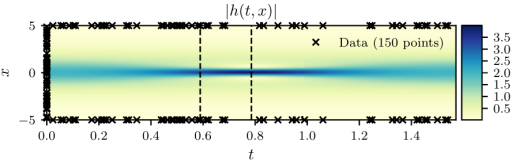
\includegraphics[width=\linewidth]{schr01}
\caption{PINN solution for the solution $h(t,x)$. The horizontal axis denotes time $t$, and the vertical axis, the coordinate $x$. The marks in the boundaries of the graph represent the randomly assigned points (BC+IC) used for training. The color scale refers to the position. The dashed vertical lines refer to 2 snapshots ($t=0.59$ and $t=0.79$).} 
\label{fig:schr1}
\end{figure}


\begin{figure}[htb]
\centering
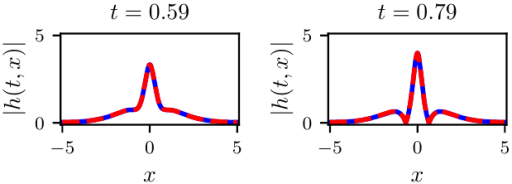
\includegraphics[width=.9\linewidth]{schr02}
\caption{Superimposed solutions for PINN and numerical solution for the $t=0.59$ and $t=0.79$ snapshots. The PINN solution is in red, and numerical solution is in blue.}
\label{fig:schr2}
\end{figure}

\begin{table}[htb]
\centering
\caption{Processing times, speedups and parallel efficiencies for the PINN  solutions for different numbers of MPI processes. The single MPI process execution time was taken as a reference. Best values are highlighted in red.}
\label{tab:resu}
\begin{tabular}{lrrrrr}\toprule											
	&	\multicolumn{5}{c}{\textbf{Number of MPI processes}}									\\
\cline{2-6}\vspace{-8pt}	&		&		&		&		&		\\
\textbf{Profiling}	&	\textbf{1}	&	\textbf{4}	&	\textbf{8}	&	\textbf{16}	&	\textbf{24}	\vspace{1pt}\\
\toprule\vspace{-10pt}	&		&		&		&		&		\\
\multicolumn{6}{c}{\textbf{\textit{Processing time (seconds)}}}											\\
\midrule[0.1pt]\vspace{-10pt}	&		&		&		&		&		\\
\textbf{Train}	&	30.33	&	22.14	&	21.69	&	22.56	&	23.21	\\
\textbf{Predict}	&	\color{red}{0.10}	&	\color{red}{0.05}	&	\color{red}{0.03}	&	\color{red}{0.03}	&	\color{red}{0.03}	\\
\toprule\vspace{-10pt}	&		&		&		&		&		\\
\multicolumn{6}{c}{\textbf{\textit{Speedup}}}											\\
\midrule[0.1pt]\vspace{-10pt}	&		&		&		&		&		\\
\textbf{Train}	&	\color{red}{1.00}	&	1.37	&	1.40	&	1.34	&	1.31	\\
\textbf{Predict}	&	\color{red}{1.00}	&	\color{red}{2.15}	&	\color{red}{3.14}	&	\color{red}{3.53}	&	\color{red}{3.65}	\\
\toprule\vspace{-10pt}	&		&		&		&		&		\\
\multicolumn{6}{c}{\textbf{\textit{Parallel efficiency}}}											\\
\midrule[0.1pt]\vspace{-10pt}	&		&		&		&		&		\\
\textbf{Train}	&	\color{red}{1.00}	&	0.34	&	0.17	&	0.08	&	0.05	\\
\textbf{Predict}	&	\color{red}{1.00}	&	\color{red}{0.54}	&	\color{red}{0.39}	&	\color{red}{0.22}	&	\color{red}{0.15}	\\
\bottomrule											
\end{tabular}																				 % the table is in Google Docs
\end{table}

\begin{figure}[htb]
\centering
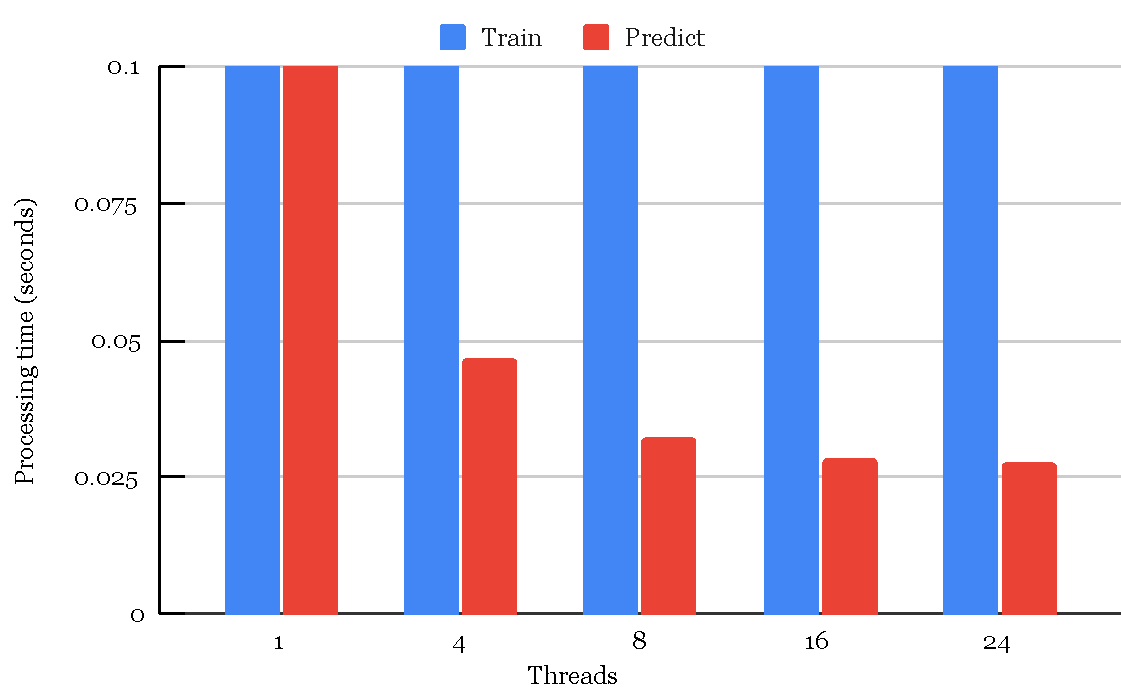
\includegraphics[width=\linewidth]{time}
\caption{Processing times (seconds) in function of number of MPI processes for the PINN implementation. "Train" refer to the PINN training phase, while "Predict" refers to the PINN test/prediction phase (for convenience, times above 0.1 seconds are not shown).}
\label{fig:time}
\end{figure}

\begin{figure}[htb]
\centering
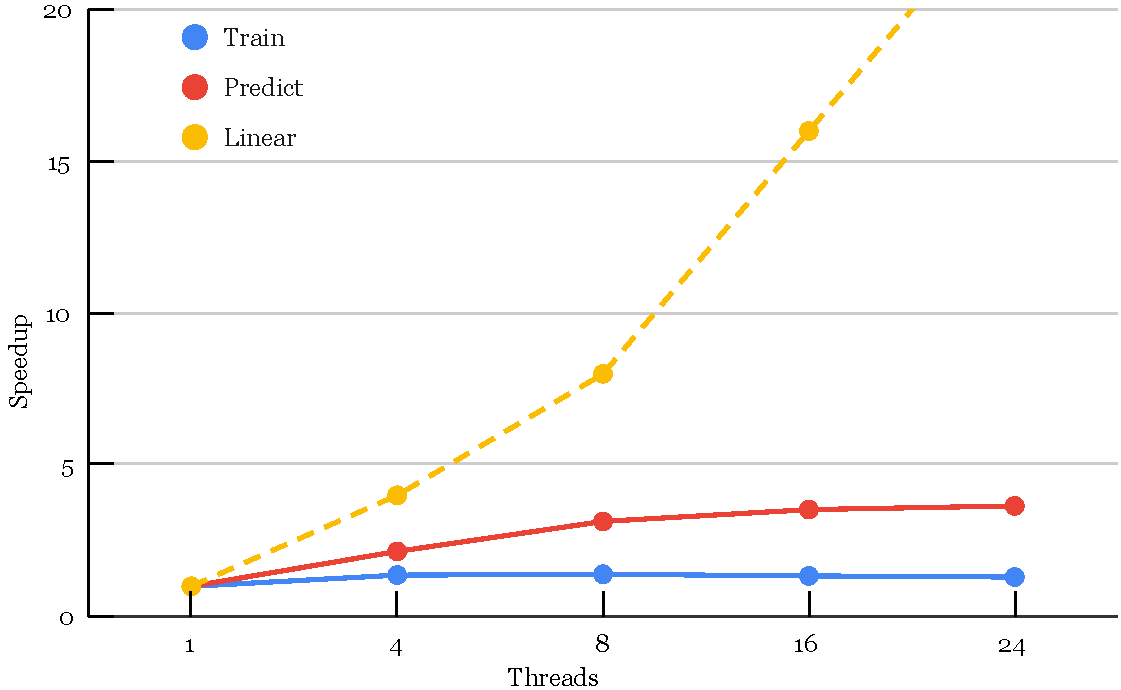
\includegraphics[width=\linewidth]{spee}
\caption{Speedups in function of the number of MPI processes for the PINN implementation. The dotted line indicates the linear speedup. "Train" refer to the PINN training phase, while "Predict" refers to the PINN test/prediction phase.}
\label{fig:spee}
\end{figure}

\begin{figure}[htb]
\centering
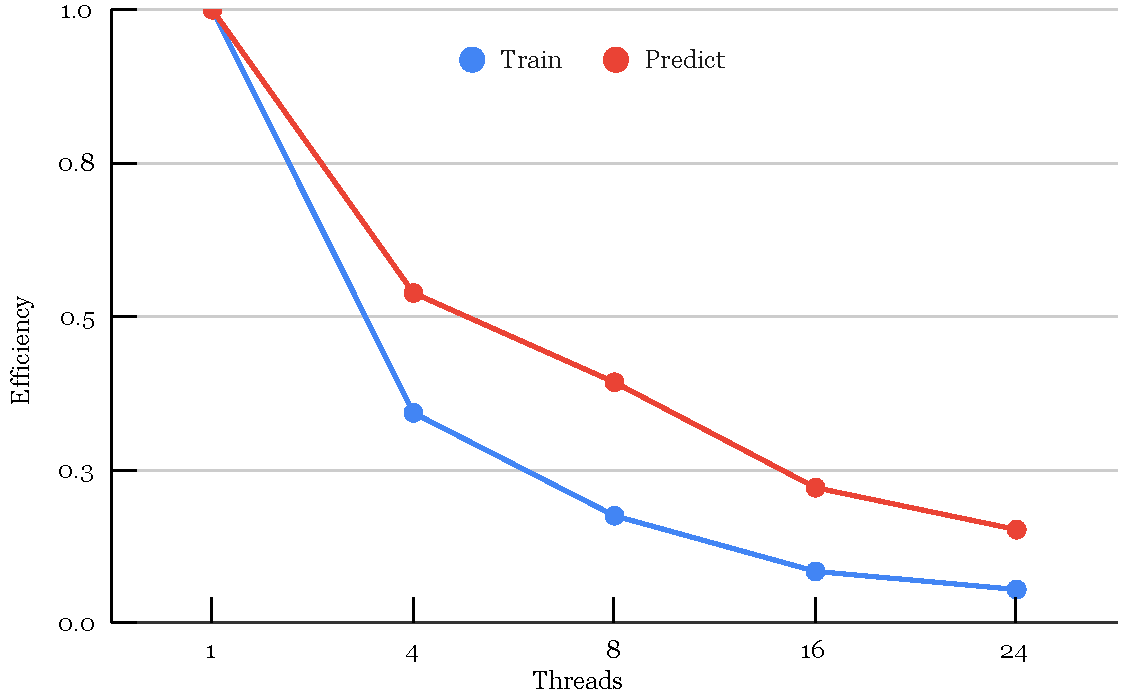
\includegraphics[width=\linewidth]{effi}
\caption{Parallel efficiencies in function of the number of OpenMP threads for the GQM and PINN implementations. "Train" refer to the PINN training phase, while "Predict" refers to the PINN test/prediction phase.}
\label{fig:effi}
\end{figure}

The \autoref{tab:resu} shows the processing times for the PINN solution. PINN time is divided into training time (Train) and prediction time (Predict). The execution time of the single MPI process, using a single GPU, without using the Horovod library, was taken as a reference. In all cases, the XXXX implementation achieved the best performance, that is, it required less processing time and presented better parallel accelerations and efficiencies, even considering only the PINN prediction time.

%
%----------------------------------------
\section{Conclusions}\label{sec:conc}
%----------------------------------------
%
This work evaluates the solution of a one-dimensional non-linear Schrodinger equation of a test problem using a Physics-Informed Neural Network (PINN), which was executed in parallel using several nodes of the SDumont computer. The Schrodinger equation is a partial differential equation (PDE) with derivatives in space and time, which is commonly solved by a numerical method. A comparison of the accuracy and required processing time of the solution running on the SDumont computer is presented for different numbers of MPI processes, each process using a single GPU. As future work, we intend to explore other PINN architectures.







% The asterisk symbol (*) is used to indicate that a environment does not produce numbering
%----------------------------------------
% \section*{References}
%----------------------------------------
%
\FloatBarrier
\bibliographystyle{IEEEtran}
\bibliography{library.bib}
%
%========================================
\end{document}
%========================================





